\textbf{Example 1}

Consider the following call:

\t{construct([[1, 1, 2, 2], [1, 1, 2, 2], [2, 2, 1, 2], [2, 2, 2, 1]])}

This means that there should be exactly one path from tower $0$ to tower $1$. For all other pairs of towers $(x, y)$, such that $0 \leq x < y \leq 3$, there should be exactly two paths from tower $x$ to tower $y$.

This can be achieved with $4$ bridges, connecting pairs of towers $(0, 1)$, $(1, 2)$, $(1, 3)$ and $(2, 3)$.

To report this solution, the \t{construct} procedure should make the following call:
\begin{itemize}
\item \t{build([[0, 1, 0, 0], [1, 0, 1, 1], [0, 1, 0, 1], [0, 1, 1, 0]])}
\end{itemize}

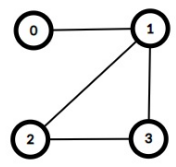
\includegraphics{Supertrees.png}

It should then return $1$.

In this case, there are multiple constructions that fit the requirements, all of which would be considered correct.

\textbf{Example 2}

Consider the following call:

\t{construct([[1, 0], [0, 1]])}

This means that there should be no way to travel between the two towers. This can only be satisfied by having no bridges.

Therefore, the \t{construct} procedure should make the following call:
\begin{itemize}
\item \t{build([[0, 0], [0, 0]])}
\end{itemize}

After which, the \t{construct} procedure should return $1$.

\textbf{Example 3}

Consider the following call:

\t{construct([[1, 3], [3, 1]])}

This means that there should be exactly $3$ paths from tower $0$ to tower $1$. This set of requirements cannot be satisfied.
As such, the \t{construct} procedure should return $0$ without making any call to \t{build}.
